
\newpage

\begin{tikzpicture}[remember picture,overlay]
  \begin{scope}[on background layer]
    \node[anchor=north west,outer sep=0,inner sep=0] (img) at (current page.north west) {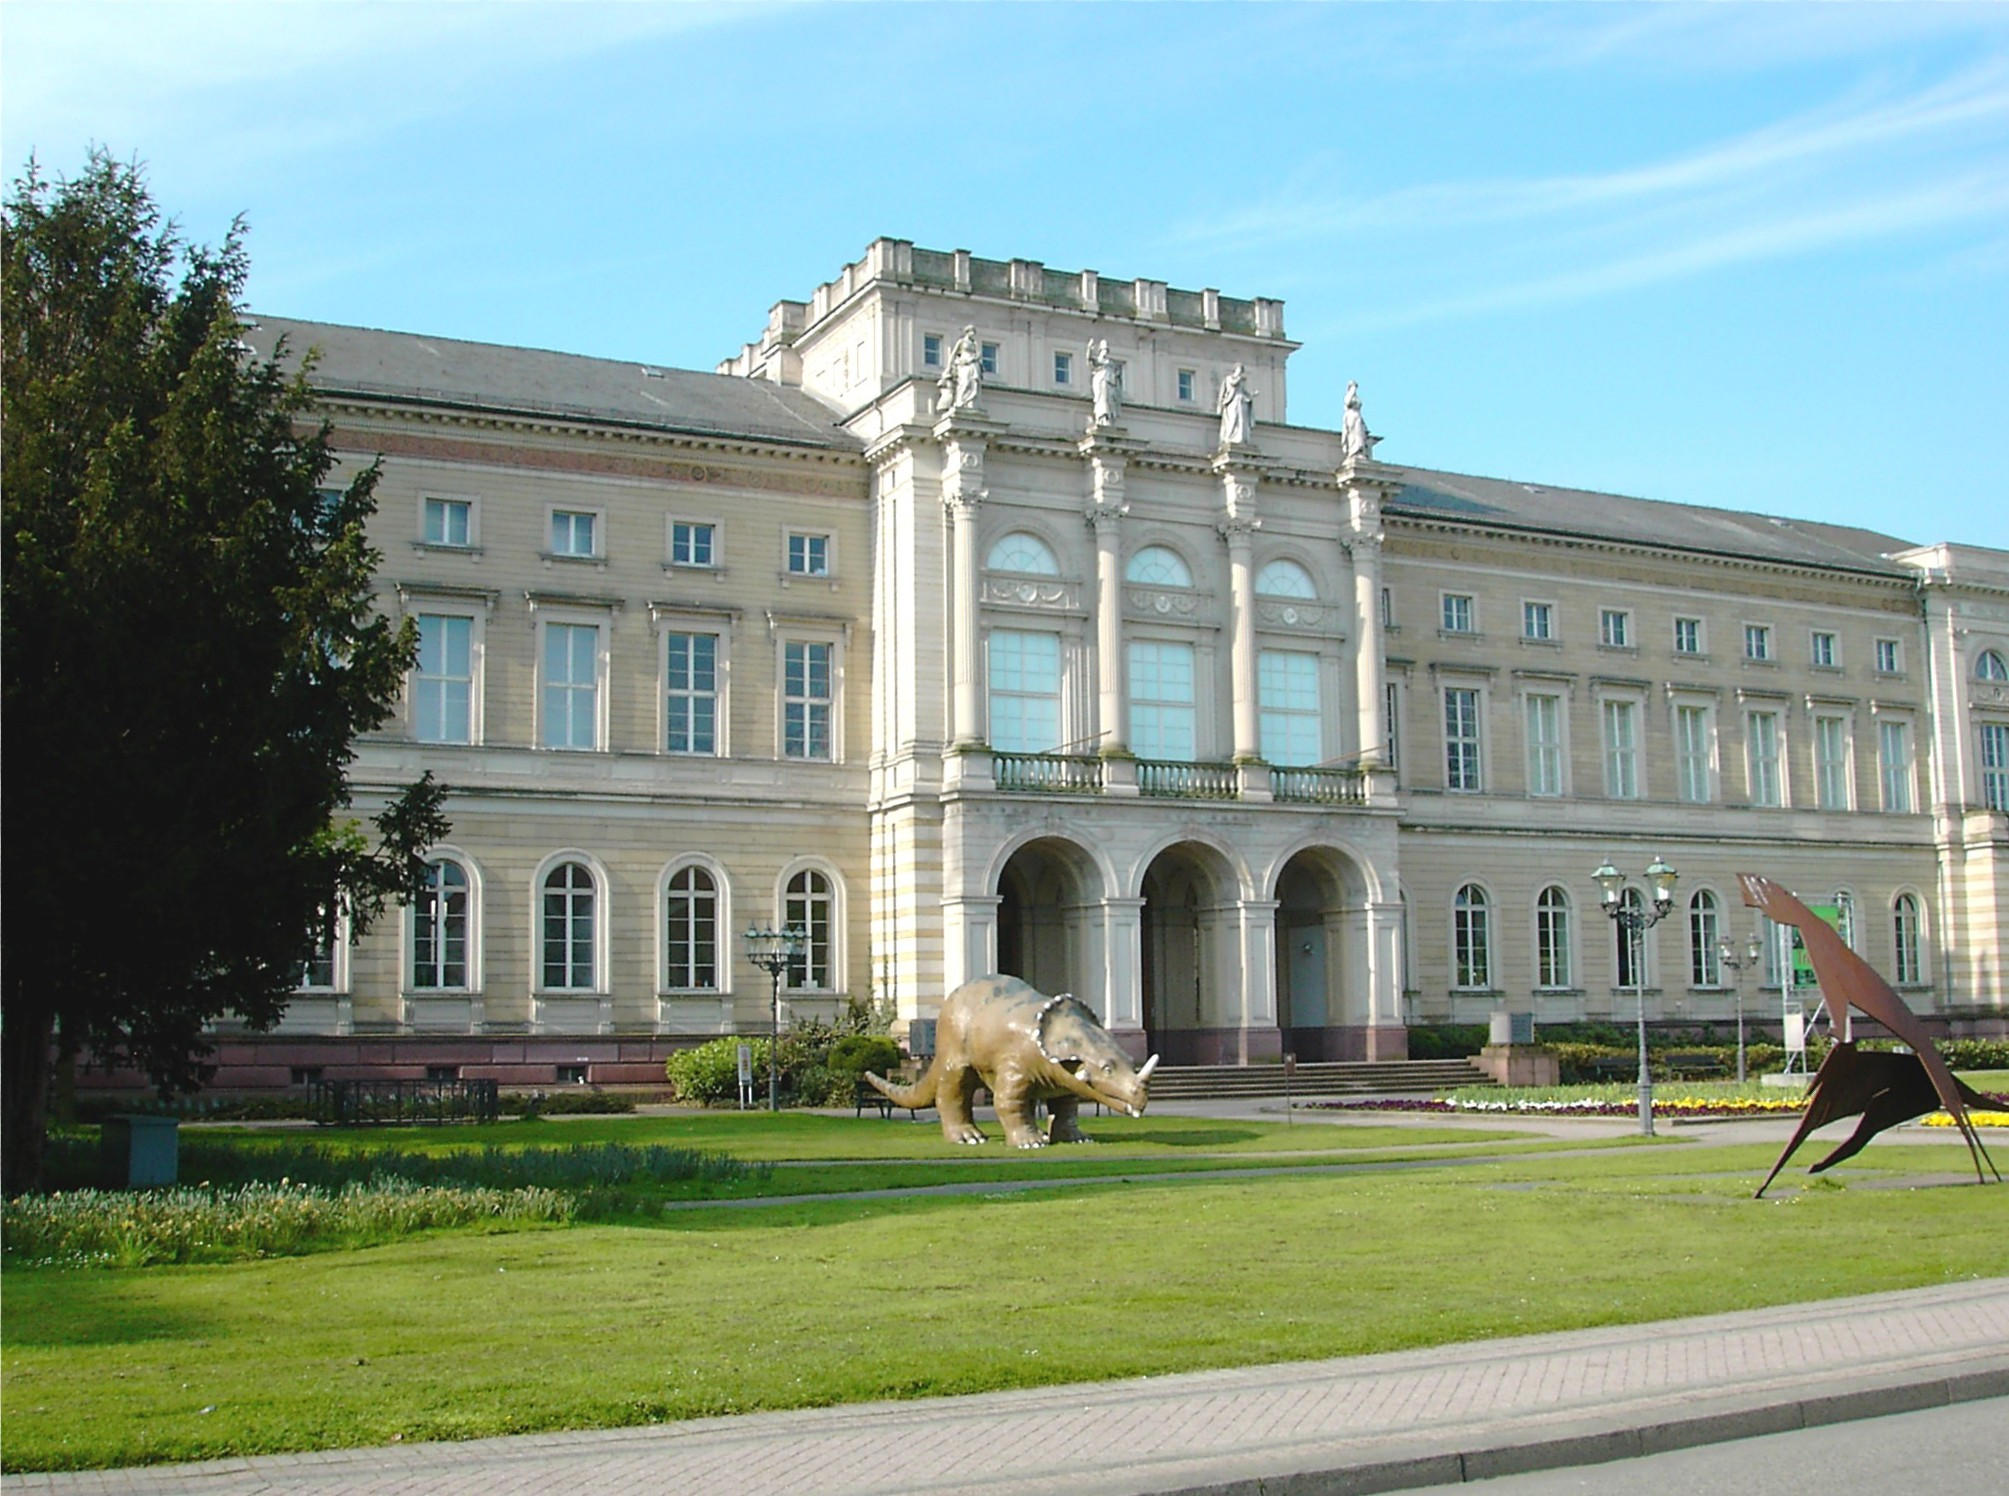
\includegraphics[width=21cm,clip,trim=0 250 0 0]{images/city/naturkundemuseum-.jpg}};
  \end{scope}
  \node[anchor=south west,color=black,xshift=1ex,yshift=1ex] (label) at (img.south west) {\imgtitle{Günter Josef Radig}{State Museum of Natural History}{CC BY-NC-SA 2.0, cropped, \url{http://ka.stadtwiki.net/Datei:Naturkundemuseum_Karlsruhe.jpg}}};
  \begin{scope}[on background layer]
    \node[fit=(label),inner sep=0,outer sep=0,opacity=0.6,fill=white,rounded corners] {};
  \end{scope}
\end{tikzpicture}

\vspace*{9.5cm}


\section{Team}

The team is currently composed of three people:
Benjamin Berg, Moira Schuler, and Tobias Mueller.

We have commitments from more people both local and remote.
We will need more help, though, and we have already discussed
what the roles and responsibilities are that need to be distributed.

Local GNOME communities are hard to find in Germany, these days,
so there is no local GNOME user group in Karlsruhe.
But there are several IT and IT friendly institutions such as the
the local CCC branch called Entropia, a FabLab, and several LUGs.
Some of those have already organized an event like GUADEC and
we hope to make use of their knowledge.

As for the legal structure supporting the event,
we consider founding registered student association at
the university to get hold of the university's resources,
but also to tap into the student's pool more easily.
We also consider founding a German non-profit which will reduce
liability for the organizers.
